\chapter{基于形变梯度的形变子空间构建}
本章将描述构建形变子空间的方法,
并给出了一个基于形变子空间的修改模型形状的算法。
形变子空间构建的输入是一个参考模型和一组形变关键帧。
本文会从每一个形变关键帧中提取出一个特征向量,
作为形变子空间的基向量。
这个特征向量描述的形变关键帧相对于参考模型的相对形变,
由模型中各三角面片的形变梯度组成。
由所有特征向量张成的空间被称为模型的形变子空间,
空间中向量均可由基向量非线性插值得到。
本文还给出了一个基于形变子空间修改模型形状的算法,
可以让用户通过拖动控制点得到符合物体形变特征模型形状。
\section{基于形变梯度的形变子空间构建}
本文基于网格模型中面片的形变梯度从形变关键帧中提取特征向量,
这些特征向量张成的空间被称作该模型的形变子空间。
本节将详细介绍形变梯度的概念,描述特征向量和网格模型互相转换的方法,
以及特征向量在非线性空间进行插值的方法。
\subsection{形变梯度}
形变梯度是一组三维点在三维空间中发生的仿射变换的雅可比矩阵。
参考模型即未发生形变的模型,在本文中即第三章中重建的三维模型。
本文描述的形变梯度是在三角面片上定义的。
将三角面片发生的仿射变换记为$\Phi$:
\begin{equation}
    \label{eq_at}
    \Phi(\bm{v})=\bm{T}\bm{v}+\bm{t}
\end{equation}
其中$3 \times 3$矩阵$\bm{T}$包含了旋转变换、缩放变换和斜切变换,
三维向量$\bm{t}$包含了三维空间中的平移变换;
$\bm{v}$为三维空间中的点。
\begin{figure}
    \centering
    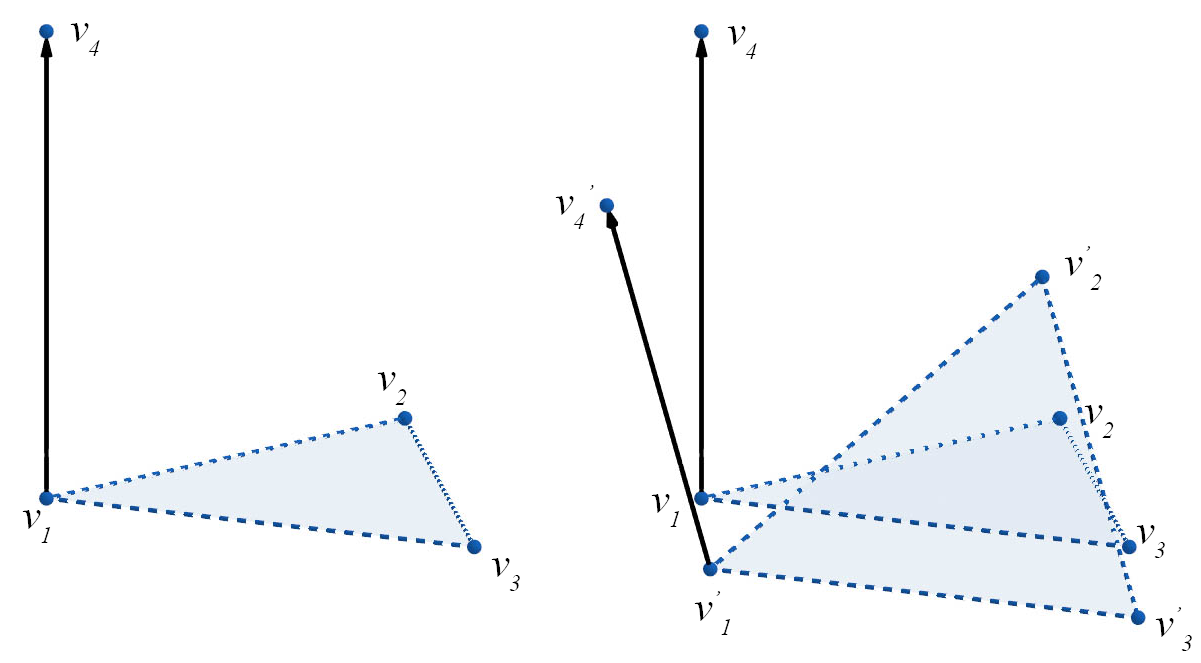
\includegraphics[width = \textwidth]{./Pictures/DefGra.png}
    \caption{}
    \label{deformation_gradient}
\end{figure}
三角面片包含三个不共线的点$\bm{v_1}$、$\bm{v_2}$、$\bm{v_3}$,
但这三个点不足以定义三维空间中的放射变换,
因为这一组点无法定义面片法线方向上的上缩放变换。
所以计算形变梯度时需要加入第四个点
\begin{equation}
    \bm{v_4}=\bm{v_1}
    +
    \frac
        {(\bm{v_2}-\bm{v_1})\times(\bm{v_3}-\bm{v_1})}
        {\sqrt{|(\bm{v_2}-\bm{v_1})\times(\bm{v_3}-\bm{v_1})|}}
\end{equation}
可以看出$\bm{v_{14}}=\bm{v_4}-\bm{v_1}$是垂直于面片的向量。
$\bm{v_{14}}$的方向通过$\bm{v_{12}}=\bm{v_2}-\bm{v_1}$和
$\bm{v_{13}}=\bm{v_3}-\bm{v_1}$的外积计算得到;
$\bm{v_{14}}$的长度为$\sqrt{|(\bm{v_2}-\bm{v_1})\times(\bm{v_3}-\bm{v_1})|}$,
这保证当面片发生仿射变换时,
$\bm{v_{14}}$会与$\bm{v_{12}}$和$\bm{v_{13}}$等比缩放。


\subsection{基于形变梯度的特征向量}
给定一个参考模型$\bm{P}$和一个形变关键帧$\bm{K}$,
它们都包含$n$个顶点和$m$个面片。
本文会从$\bm{K}$提取一个相对于$\bm{P}$的特征向量。
\subsection{特征向量的非线性插值}
\section{基于形变子空间的网格模型形状修改}
\section{本章小结}